\documentclass[11pt]{article}

\usepackage{setspace}
\usepackage{amsmath}
\usepackage{enumitem}
\usepackage{amsfonts} 
\usepackage{mathtools}
\usepackage{relsize}
\usepackage{graphicx}
\usepackage[top=2cm,bottom=2cm,left=2.5cm,right=2.5cm,marginparwidth=1.75cm]{geometry}
\setlength{\parindent}{0cm}
\usepackage{listings}
\usepackage{clrscode3e}
\usepackage{graphicx}
\def \n {\par \vspace{\baselineskip}}

\def\lc{\left\lceil}   
\def\rc{\right\rceil}
\def\lf{\left\lfloor}   
\def\rf{\right\rfloor}

\title{\vspace{-1.0cm}PHYS 2303 Homework 4}
\author{Fletcher Gornick}
\date{February 15, 2022}

\spacing{1.5}
\begin{document}
 \maketitle 
 \section*{Chapter 16 Problem 69}
 Two strings are attached between two poles separated by a distance of 2.00 m as shown below, both under the same tension of 600.00 N. 
 String 1 has a linear density of \(\mu_1\) = 0.0025 kg/m and string 2 has a linear mass density of \(\mu_2\) = 0.0035 kg/m. Transverse 
 wave pulses are generated simultaneously at opposite ends of the strings. How much time passes before the pulses pass one another? \\

 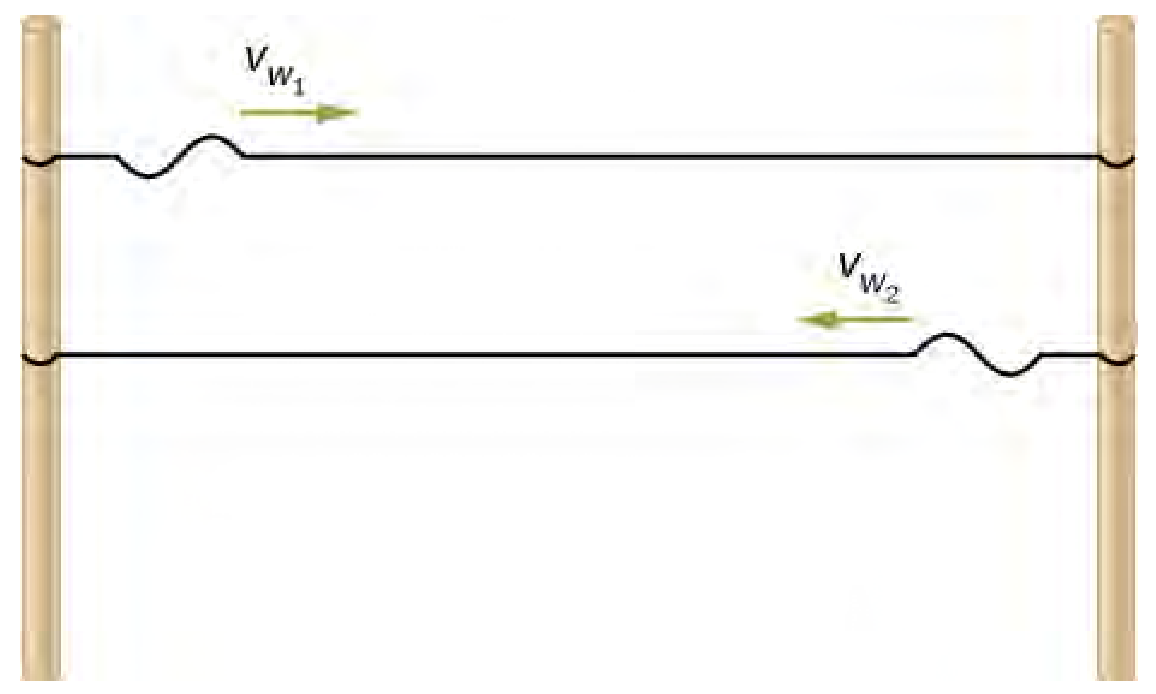
\includegraphics[scale=0.35]{16-69.png}
 \newpage

 \section*{Chapter 16 Problem 104}
  Consider the experimental setup shown below. The length of the string between the string vibrator and the pulley is \(L\) = 1.00 m. The 
  linear density of the string is \(\mu\) = 0.006 kg/m. The string vibrator can oscillate at any frequency. The hanging mass is 2.00 kg. \\

  (a) What are the wavelength and frequency of \(n\) = 6 mode? \\

  (b) The string oscillates the air around the string. What is the wavelength of the sound if the speed of the sound is \(v_s\) = 343.00 m/s?

 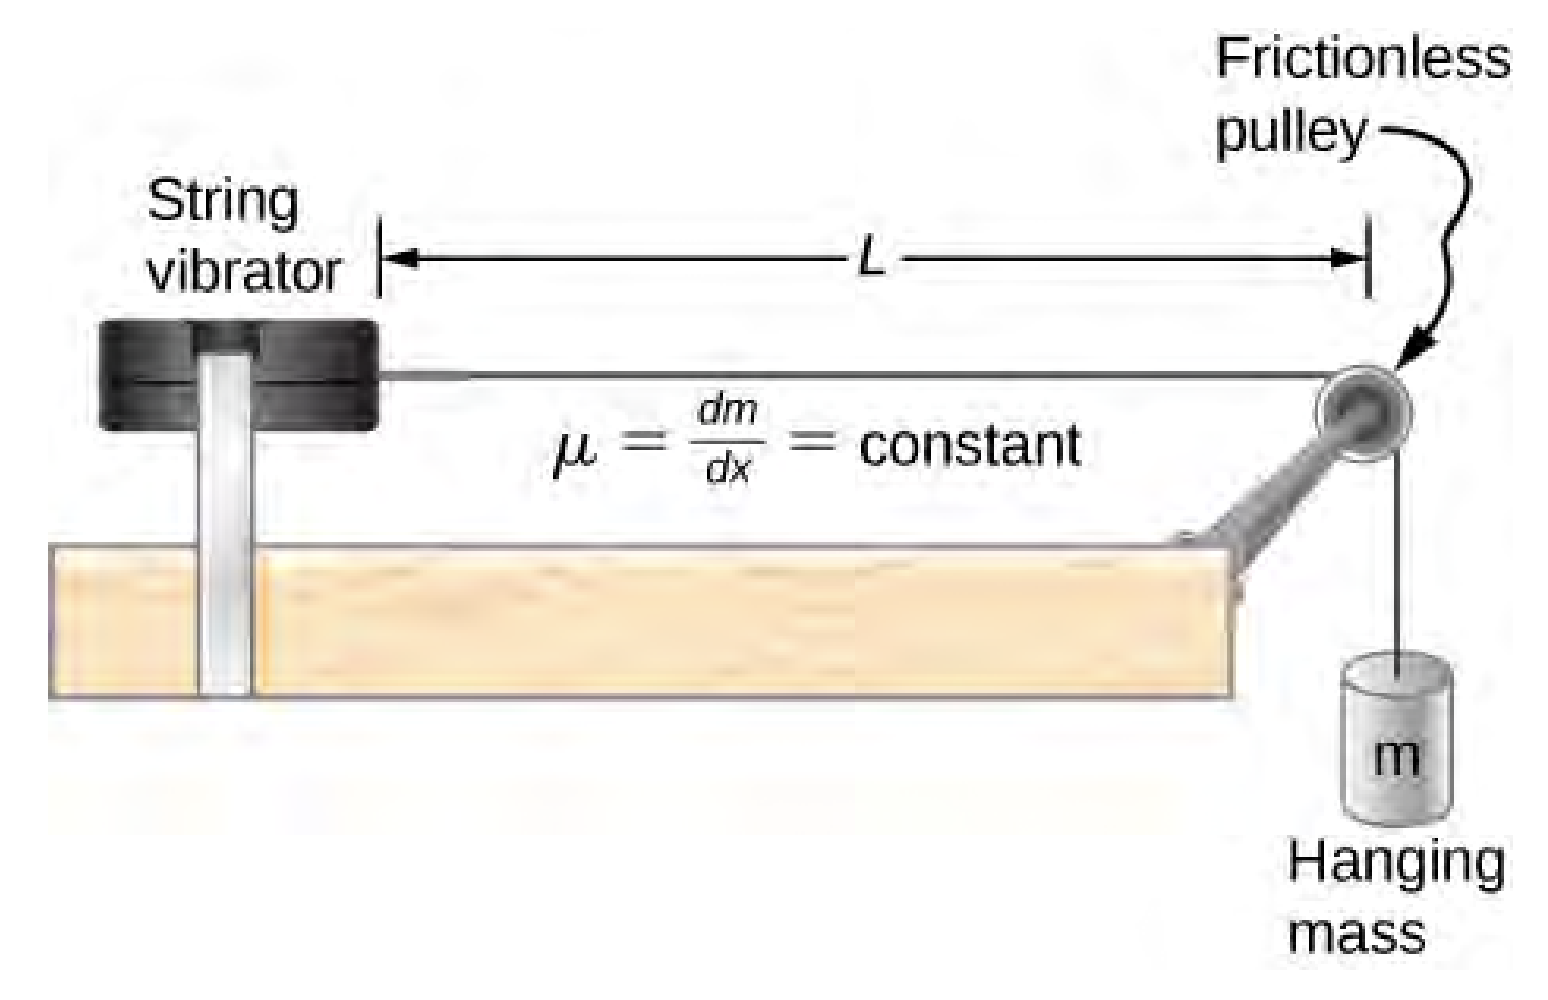
\includegraphics[scale=0.35]{16-104.png}
 \newpage

 \section*{Chapter 16 Problem 146}
 A string with a linear mass density of \(\mu\) = 0.0085 kg/m is fixed at both ends. A 5.0-kg mass is hung from the string, as shown below. 
 If a pulse is sent along section A, what is the wave speed in section A and the wave speed in section B? \\

 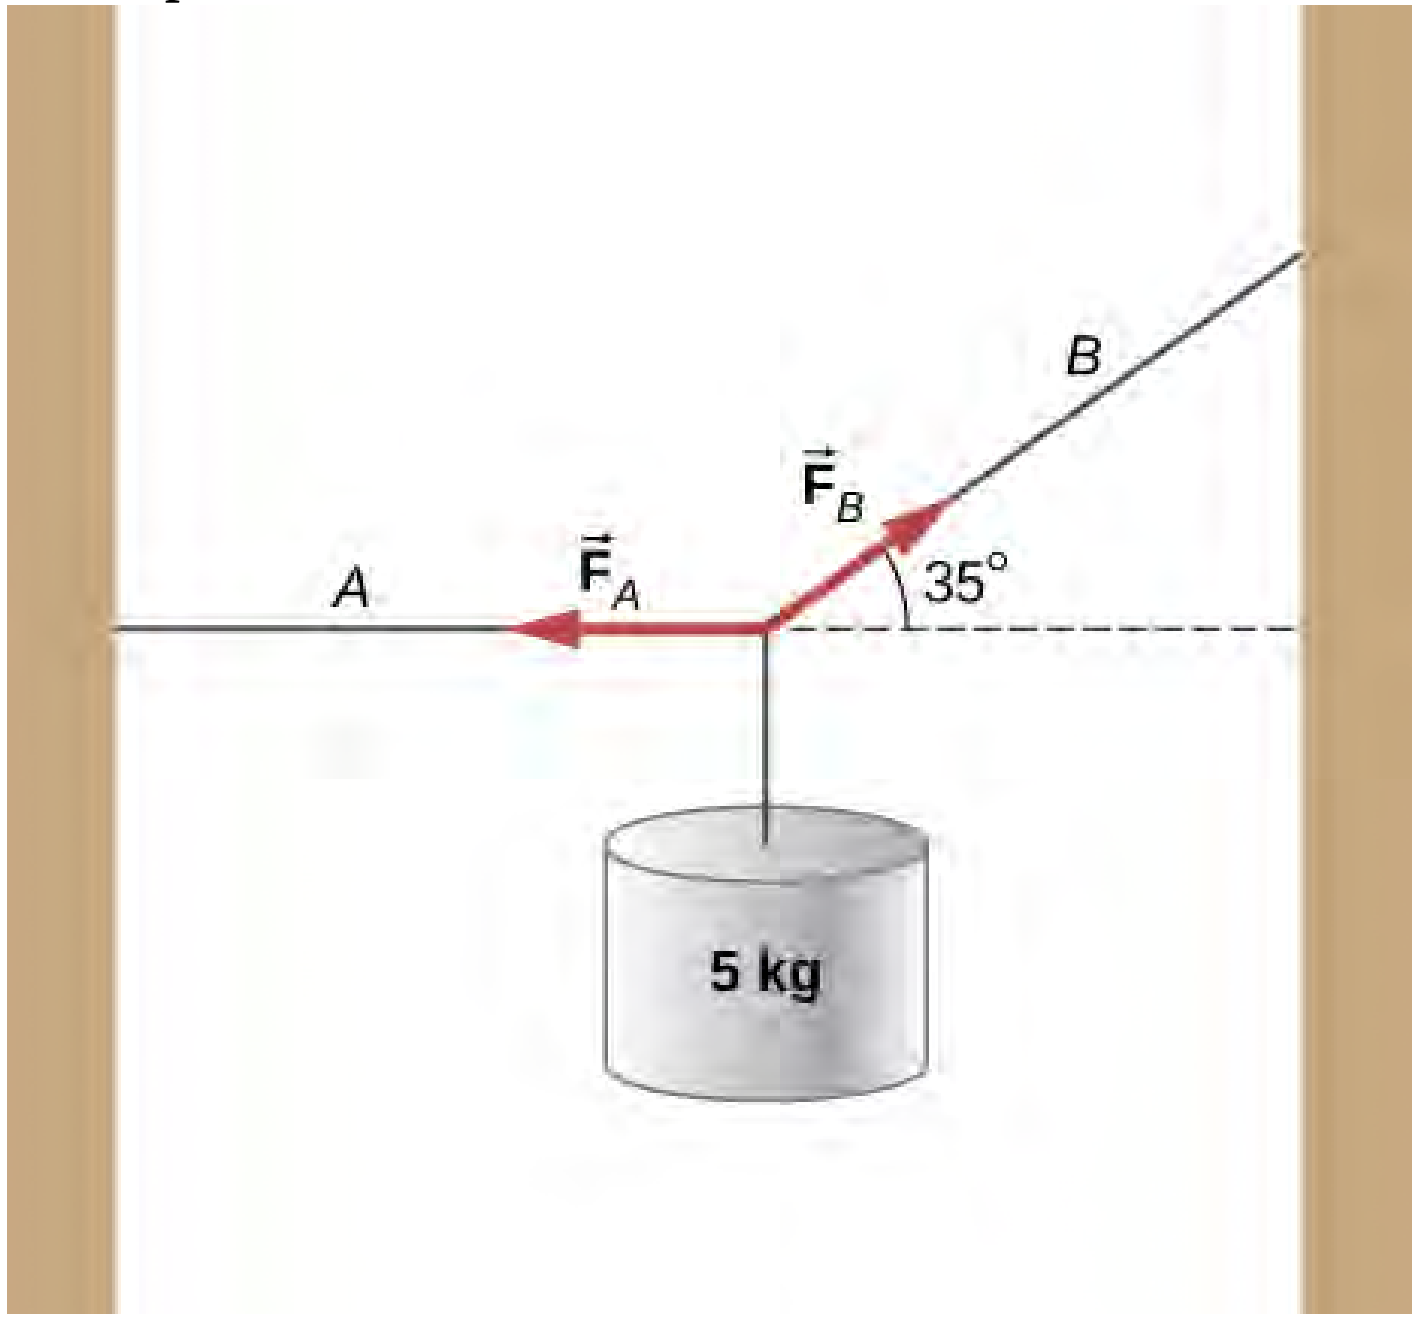
\includegraphics[scale=0.35]{16-146.png}

\end{document}
